%!TEX root = ../main.tex
\subsubsection{Compact spaces}
The last property that we will discuss is compactness. It will be discussed for both topological and metric spaces. We now provide some basic definition specific for topological space, even if those make sense for metric spaces also.

\begin{defn}\label{compact-space-defn}
	Let $(X,\tau)$ be a topological space
	and $E\subset X$.\\
    A family $\{E_i\}_{i\in I}$ is a \emph{cover} of $E$
    if 
    $$
    	E 
    	\subset \bigcup_{i \in I} E_i 
    .
    $$
    An \emph{open cover} is a cover made of open sets.\\
    A \emph{subcover} is a subfamily of a cover which is a cover of $E$ itself.
    That is, $\{E_i\}_{i\in J}$, $J \subset I$,
    is a subcover if $E \subset \bigcup_{i\in J} E_i$.
\end{defn}

\begin{defn}
	Let $(X, \tau)$ be a topological space.
    The set $X$ is \emph{compact}
    if from each of its open cover, we can select a finite subcover. Namely:
    $$
    	\forall \{A_i\}_{i\in I}, 
    	\ A_i \in \tau 
    	\ \forall i \in I 
    	\ : \ X \subset \bigcup_{i\in I} A_i; 
    	\ \exists \, J \subset I, J \ \text{finite}
    	\ : \ X \subset \bigcup_{i \in J} A_i
    .
    $$
\end{defn}

In case of single set withing a topological spaces, we have the following

\begin{defn}
	Let $(X,\tau)$ be a topological space
	and $E\subset X$.\\
	We say that $E$ is \emph{compact} if it is compact as topological space with the induced topology\footnotemark{},
	that is every cover of $E$ made of open sets of $X$ admits a finite subcover.
\end{defn}
\footnotetext{An induced topology for a set belonging to a topological space is the smallest topology for which any subset open with respect the topology of the space is open.}

Notice that if $\tau_1$ and $\tau_2$ are topologies on $X$, with $\tau_2$ weaker than $\tau_1$, and $E \subset X$ is compact with respect to $\tau_1$, then $E$ is also compact with respect to $\tau_2$; the reverse is false.

\begin{exam}
	The set $E=(0,1)$ is not compact with respect to $d_e$.\\
	Indeed, consider $E_n = (\frac 1 n, 1)$, which is open: $\{E_n\}$ is a cover for $E$ as $(0,1) \subset \bigcup_{n\in \NN} E_n$, but there is no finite subcover.
\end{exam}
\begin{exam}	
	Consider $(X, \tau_d)$, where $\tau_d$ is the discrete topology for which all subset of $X$ are open ($\tau_d = \Pc(X))$: only finite subsets of $X$ are compact.
\end{exam}
\begin{exam}	
	Consider $(X, \tau_0)$ with $\tau_0 = \{\varnothing, X\}$: any subset of $X$ is compact.
\end{exam}

\begin{prop}
    Let $(X, \tau)$ be a compact topological space and $S \subseteq X$.\\
    If $S$ is closed then $S$ is compact.
\end{prop}
\begin{proof}
    Let $\{E_i\}_{i\in I}$ be a cover of $S$ made of open sets in $X$.\\
    As if $S$ is closed then $X\setminus S$ is open,
    $\{E_i\}_{i\in I} \cup (X \setminus S)$ is an open cover of $X$.\\
	Since $(X, \tau)$ is compact, this open cover admits a finite subcover, that is:
	$$\exists \, J \subset I : \quad X \subset (\cup_{j \in J} E_j) \cup (X \setminus S).$$
	So $S \subset \cup_{j \in J} E_j$, that is $\{E_j\}_{j \in J}$ is a finite subcover of $S$, hence the thesis.
\end{proof}

Notice that the compactness of $S$ does not imply the closedness of $S$; for example in $(X, \tau_0)$ only $X$ and $\varnothing$ are closed, yet any $A\subset X$ is compact. 

Now the reader could prove this proposition.
\begin{prop}
	Continuous functions map compact sets into compact sets.
\end{prop}
    
\paragraph{Sequentially compactness} We can provide a slightly different definition or compactness, again we provide the definition for topological spaces but it take sense for metric spaces as well.
    
\begin{defn}\label{seq-compact-space-defn}
	We say that $(X, \tau)$ is \emph{sequentially compact} if for every sequence in $X$ it exists a convergent subsequence, namely: 
	$$\forall \{x_n\} \subset X \quad \exists \, \{ x_{n_k} \} \subset X : \quad x_{n_k} \xrightarrow{k\to\infty} x^\star \in X.$$ 
\end{defn}

Compactness and sequential compactness are different notions, and they do not imply each other, but there are some relations. Indeed, for topological spaces the following theorems hold (recall definition of first and second countable spaces \vref{first-second-countable}):

\begin{theo}
	Let $(X,\tau)$ be a topological space, let $E\subset X$ compact.\\
	If $X$ is first countable, then $E$ is sequentially compact.
\end{theo}

\begin{theo}
	Let $(X, \tau)$ be a topological space, let $E\subset X$ be sequentially compact.\\
	If $X$ is second countable, then $E$ is compact.
\end{theo}

\paragraph{Compactness for metric spaces} In metric spaces the notion of compactness is the same as for topological spaces; indeed, it is defined upon the notion of openness, which has already been defined for both kind of spaces. Here we see the relation between compactness and boundedness for metric spaces (recall definition of totally bounded set \vref{metric-totally-bounded}).
    
\begin{theo}[Characterization of compact spaces]\label{characterization-compact-spaces}
    If $(X,d)$ is a metric space, the following are equivalent:
    \begin{itemize}
        \item the set $X$ is compact;
        \item the set $X$ is sequentially compact;
        \item the set $X$ is complete and totally bounded.
    \end{itemize}
\end{theo}

\begin{coro}
	Let $(X,d)$ be a metric space, with $E \subset X$.\\
	If $E$ is compact then it is closed and bounded.
\end{coro}

\begin{proof}
	First, as $E$ is compact, then it is totally bounded, so it is also bounded: see the previous theorem.
	
	Let us prove that $E$ is closed: it's enough to show that $E$ is sequentially closed.\\
	By the previous theorem, if $E$ is compact then it is also complete.\\
	Take a converging sequence $\{x_n\}_{n\in \NN} \subset E$ such that $x_n \xrightarrow{d} x^\star$. Is $x^\star \in E$?\\
	Since $\{x_n\}_{n\in \NN}$ is fundamental (it's converging) and $E$ is complete, $\{x_n\}_{n\in \NN}$ has a limit in $E$ so $x^\star \in E$ and the thesis is reached.
\end{proof}

The converse in general is not true.

\paragraph{Heine--Borel theorem} In case of $X=\RR^N$ we have the following important theorem:

\begin{theo}[Heine--Borel]\label{heine-borel-theo}
	Let $(\RR^N, d_e)$ and $K \subset \RR^N$. \\
	Then $K$ is compact if and only if $K$ is closed and bounded
\end{theo}
As in later chapters compact set will play a important role, we denote a compact set with the letter $K$.

\begin{proof}
	\textit{Necessary condition} $\implies$:\\
	This follows from the previous corollary.
	
	\textit{Sufficient condition} $\impliedby$:\\
	As $K\subset \RR^N$ is closed and $\RR^N$ complete, $K$ is complete as well.\\
	Consider an hypercube $C$ such that $C\supset K$ with $l$ being the length of its side, divide $C$ into $m^n$ small cubes, with $m \in \NN$ which have size $\frac l m$.\\
	Let's call them 
	$$
		C_1^{(m)}, \ldots , C_m^{(m)}
	.
	$$
	Their diagonal has length $d_m = \frac l m \sqrt{n}\xrightarrow{m\to\infty}0$.\\
	Now fix $\varepsilon>0$ and take $m$ large such that $d_m < \varepsilon$. Then:
	$$
		K 
		\subset C 
		= \bigcup_{j=1}^{m^n} C_j^{(m)}
		\subset \bigcup_{j=1}^{m^n} B_\varepsilon(x_j)
	.
	$$
	So the set is totally bounded and complete, therefore it is also compact, hence the thesis.
\end{proof}

This \textit{does not work in infinite dimensional spaces} because $m^n \xrightarrow{n\to\infty} + \infty$ and total boundedness requires a finite amount of balls.

\paragraph{Function defined on compact spaces}

\begin{prop}
	Let $(X, \tau_x)$ and $(Y, \tau_y)$ two topological spaces and $E \subset X$ be compact. Let $f:X\to Y$ be a continuous function.\\
	Then the image $f(E)$ compact.
\end{prop}
\begin{proof}
	Let $\{ B_i \}_{i \in I}$ be an open cover of $f(E)$, and $A_i \coloneqq f^{-1}(B_i)$.\\
	Then $A_i$ is open (from the continuity of $f$) and $E \subset \bigcup_{i \in I}A_i$.\\
	As $E$ is compact, it exists a finite subcover $E\subset \bigcup_{k=1}^{n} A_{i_k}$. This implies that:
	$$f(E) \subset f\left(\bigcup_{c=1}^m A_{i_k} \right) = \bigcup_{k=1}^n B_{i_k}$$
	which is a finite subcover of $f(E)$, so it's compact.
\end{proof}

\begin{theo}[Weierstrass]
	Let $(X, \tau)$ topological space, $X$ compact, and $f:X \to \RR$ continuous.\\
	Then $F$ achieves a maximum and a minimum.
\end{theo}
\begin{proof}
	The image $f(X) \in \RR$ is compact, so it's closed and bounded.\\
	This implies that $\sup f(x) \subset f(X)$ and $\inf f(x) \subset f(X)$.\\
	So there exists a maximum and a minimum.
\end{proof}

\paragraph{Semicontinuity} Now we define a weaker notion of continuity (see definition of limsum and liminf \vref{liminf-limsup-defn}).

\begin{defn}
	Let $(X,\tau)$ a topological space, and let $f : X \to \RR^\star$.\\
	We say that $f$ is \emph{lower semicontinuous} in $x_0 \in X$ if:
	$$\forall \varepsilon > 0 \quad \exists \, U \in \tau : \quad x_0 \in U  \text{ and } f(x) > f(x_0)- \varepsilon \quad \forall x \in U.$$
	Equivalently in a metric space $(X, d)$, $f$ is lower semicontinuous if:
	$$\liminf\limits_{x \to x_0} f(x) \geq f(x_0).$$

	We say that $f$ is \emph{upper semicontinuous} in $x_0 \in X$ if:
	$$\forall \varepsilon > 0 \quad \exists \, U \in \tau : \quad x_0 \in U  \text{ and } f(x) < f(x_0)- \varepsilon \quad \forall x \in U.$$
	Equivalently in a metric space $(X, d)$, $f$ is upper semicontinuous if:
	$$\limsup\limits_{x \to x_0} f(x) \leq f(x_0).$$
\end{defn}
Observe that $f$ is continuous if and only if it is both lower semicontinuous and upper semicontinuous; as it happens with the existence of the limit.

\begin{figure}[htpb]
	\centering
	\hspace{\fill}
	\begin{subfigure}{0.3\textwidth}
		\centering
		\tikzset{every picture/.style={line width=0.75pt}} %set default line width to 0.75pt        
		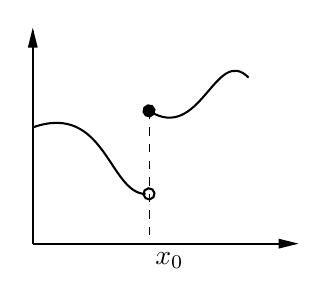
\begin{tikzpicture}[x=0.75pt,y=0.75pt,yscale=-0.8,xscale=0.8]
			\draw (40,220) -- (198,220);
			\draw [shift={(200,220)}, rotate = 180] [fill={rgb, 255:red, 0; green, 0; blue, 0 }  ][line width=0.08]  [draw opacity=0] (12,-3) -- (0,0) -- (12,3) -- cycle;
			\draw (40,220) -- (40,92);
			\draw [shift={(40,90)}, rotate = 90] [fill={rgb, 255:red, 0; green, 0; blue, 0 }  ][line width=0.08]  [draw opacity=0] (12,-3) -- (0,0) -- (12,3) -- cycle;
			\draw (40,150) .. controls (83.65,134.48) and (85.9,189.53) .. (107.9,190.11);
			\draw [shift={(110,190)}, rotate = 352.87] [color={rgb, 255:red, 0; green, 0; blue, 0 }  ][line width=0.75] (0, 0) circle [x radius= 3.35, y radius= 3.35];
			\draw (170,120) .. controls (150,100) and (141,160) .. (110,140);
			\draw [shift={(110,140)}, rotate = 212.83] [color={rgb, 255:red, 0; green, 0; blue, 0 }  ][fill={rgb, 255:red, 0; green, 0; blue, 0 }  ][line width=0.75] (0, 0) circle [x radius= 3.35, y radius= 3.35];
			\draw [dashed, very thin]  (110,140) -- (110,220);
			\draw (112,223.4) node [anchor=north west][inner sep=0.75pt]    {$x_0$};
		\end{tikzpicture}
		\caption{u.s.c.}
	\end{subfigure}
	\begin{subfigure}{0.3\textwidth}
		\centering
		\tikzset{every picture/.style={line width=0.75pt}} %set default line width to 0.75pt        
		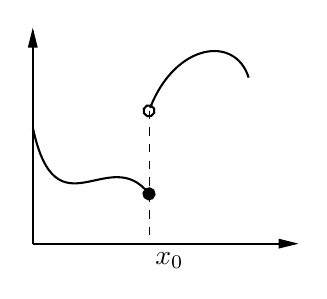
\begin{tikzpicture}[x=0.75pt,y=0.75pt,yscale=-0.8,xscale=0.8]
			\draw (260,182) -- (418,182);
			\draw [shift={(420,182)}, rotate = 180] [fill={rgb, 255:red, 0; green, 0; blue, 0 }  ][line width=0.08]  [draw opacity=0] (12,-3) -- (0,0) -- (12,3) -- cycle;
			\draw (260,182) -- (260,54);
			\draw [shift={(260,52)}, rotate = 90] [fill={rgb, 255:red, 0; green, 0; blue, 0 }  ][line width=0.08]  [draw opacity=0] (12,-3) -- (0,0) -- (12,3) -- cycle;
			\draw (260,112) .. controls (274,178) and (306,121) .. (330,152);
			\draw [shift={(330,152)}, rotate = 52.25] [color={rgb, 255:red, 0; green, 0; blue, 0 }  ][fill={rgb, 255:red, 0; green, 0; blue, 0 }  ][line width=0.75] (0, 0) circle [x radius= 3.35, y radius= 3.35];
			\draw (390,82) .. controls (382.12,56.39) and (346.1,60.86) .. (330.69,100.18);
			\draw [shift={(330,102)}, rotate = 110.1] [color={rgb, 255:red, 0; green, 0; blue, 0 }  ][line width=0.75] (0, 0) circle [x radius= 3.35, y radius= 3.35];
			\draw [dashed, very thin]  (330,102) -- (330,182);
			\draw (332,185.4) node [anchor=north west][inner sep=0.75pt]    {$x_0$};
		\end{tikzpicture}
		\caption{l.s.c.}
	\end{subfigure}
	\begin{subfigure}{0.3\textwidth}
		\centering
		\tikzset{every picture/.style={line width=0.75pt}} %set default line width to 0.75pt        
		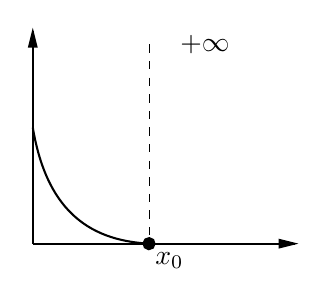
\begin{tikzpicture}[x=0.75pt,y=0.75pt,yscale=-0.8,xscale=0.8]
			\draw (434,208) -- (592,208);
			\draw [shift={(594,208)}, rotate = 180] [fill={rgb, 255:red, 0; green, 0; blue, 0 }  ][line width=0.08]  [draw opacity=0] (12,-3) -- (0,0) -- (12,3) -- cycle;
			\draw (434,208) -- (434,80);
			\draw [shift={(434,78)}, rotate = 90] [fill={rgb, 255:red, 0; green, 0; blue, 0 }  ][line width=0.08]  [draw opacity=0] (12,-3) -- (0,0) -- (12,3) -- cycle;
			\draw (434,138) .. controls (442,186) and (466,206) .. (504,208);
			\draw [shift={(504,208)}, rotate = 3.01] [color={rgb, 255:red, 0; green, 0; blue, 0 }  ][fill={rgb, 255:red, 0; green, 0; blue, 0 }  ][line width=0.75]   (0, 0) circle [x radius= 3.35, y radius= 3.35];
			\draw [dashed, very thin]  (504,88) -- (504,208);
			\draw (506,211.4) node [anchor=north west][inner sep=0.75pt]    {$x_0$};
			\draw (521,80.4) node [anchor=north west][inner sep=0.75pt]    {$+\infty $};
		\end{tikzpicture}
		\caption{l.s.c.}
	\end{subfigure}
	\hspace{\fill}
	\caption{Examples of lower and upper semicontinuous functions.}
\end{figure}
\FloatBarrier

\begin{theo}
	Let $f:(X,\tau) \to \RR$ a lower semicontinuous function defined on a topological space, with $X$ compact.\\
	Then $f$ achieves its minimum.
	
	Let $f:(X,\tau) \to \RR$ an upper semicontinuous function defined on a topological space, with $X$ compact.\\
	Then $f$ achieves its maximum.
\end{theo}

Now some results to complete the treatise.

\begin{theo}[Cantor's intersection theorem II]
	Let $(X,d)$ be a topological space, $\{K_n\}_{n\in\NN}$ be a sequence of compact sets with $K_{n+1} \subset K_n$ and $K_n \neq \varnothing \quad \forall n \in \NN$.\\
	Then $$\bigcap_{n \in \NN} K_n  \neq \varnothing.$$
\end{theo}

\begin{theo}[Heine--Cantor] \label{Heine-Cantor-theorem}
	Let $(X,d)$ be a metric space, $X$ a compact set and $f:X \to \RR$ a continuous.\\
	Then $f$ is uniformly continuous.
\end{theo}


